\documentclass[../main.tex]{subfiles}
\begin{document}

\section{Notation \& Definitions}
In this section we introduce a mathematical description of the visualization pipeline where artist $A$ functions transform data of type $\Gamma(E)$ to an intermediate representation in prerendered display space of type $\Gamma(H)$:

\begin{equation}
    A: \Gamma(E) \rightarrow \Gamma(H)
    \lab{eq:artist}
\end{equation}

\begin{enumerate}
\item $A$ is the function that converts an instance of data $\Gamma(E)$ to an instance of a visual representation $\Gamma(H)$ 
\item $E$ is a locally trivial fiber bundle over $K$ representing data space.
\item $K$ is a triangulizable space encoding the connectivity of the observations in the data. 
\item $H$ is a fiber bundle over $S$ representing visual space
\item $S$ is a simplacial complex of triangles encoding the connectivity of the visualization of $\Gamma(E)$
\end{enumerate}

When E is a trivial fiber bundle $E = F \times K$, it can be assumed that all $F_{k}$ for $k \in K$ are equal. Fiber bundles are product spaces of toplological spaces, which are a set of points with a set of neighborhoods for each point\cite{some topology text book, really wikipedia}.


\subsection{Data Model}
\begin{figure}[ht]
    \label{fig:fiberbundle}
    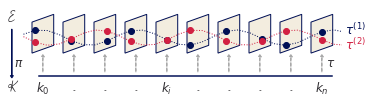
\includegraphics{figures/sections/math/fiberbundle.png}
    \caption{write up some words here}

    %% simpler still replace w/ timeseries of temp, 1D fiber -> inspired by butler 1989 FIgG 1
\end{figure}

We use a fiber bundle model to represent the data, as proposed by Butler 
\cite{butlerVectorBundleClassesForm1992,butlerVisualizationModelBased1989}. A fiber bundle is a topological total space $E$ with an embedded fiber space $F$, a base space on which the fibers lie $K$ and the $\pi$ and $\sigma$ mappings between $E$ and $K$. 

\begin{tikzcd}
    F \arrow[r, hook] & E \arrow[d, "\pi" description, bend right ] \\
                      & K \arrow[u, description, bend right]
\end{tikzcd}

As illustrated by figure~\ref{fig:fiberbundle}, the vertical lines $F$ are the range of possible temperature values embedded in the total space $E$. The base space $K$ of the fiber bundle describes the connectivity of the points in $E$; in figure~\ref{fig:fiberbundle} the connectivty of the timeseries is encoded in the line representation of $K$. The function $\pi$ is the mapping from a point on a specific fiber $F_{k}|k\in K$ in $E$ to a location $k \in K$. 
The section $\sigma$ is the mapping from locations $k$ on $K$ to points on $F_{k}$ in $E$.
%%% include diagram here of formal definition of sigma

The space of all $\sigma$ is $\Gamma$  (Pull this back into more specific about fig, the general is making this more confusing.)
%% locally trivial - for every point in K there exists an open set neighborhood $U$ such that if you restrict E to that point, then  \iota*E = F\times U [maybe do mobius strip diagram here? U is subsection of the ring, part where it's not twisted. there exists a triangulation & a way to do so is simplicies

\subsubsection{Base Space $K$}
\begin{figure}
    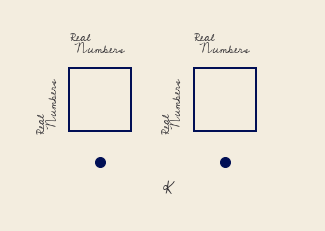
\includegraphics{figures/sections/math/temp_1k.png}
\end{figure}
\begin{figure}
    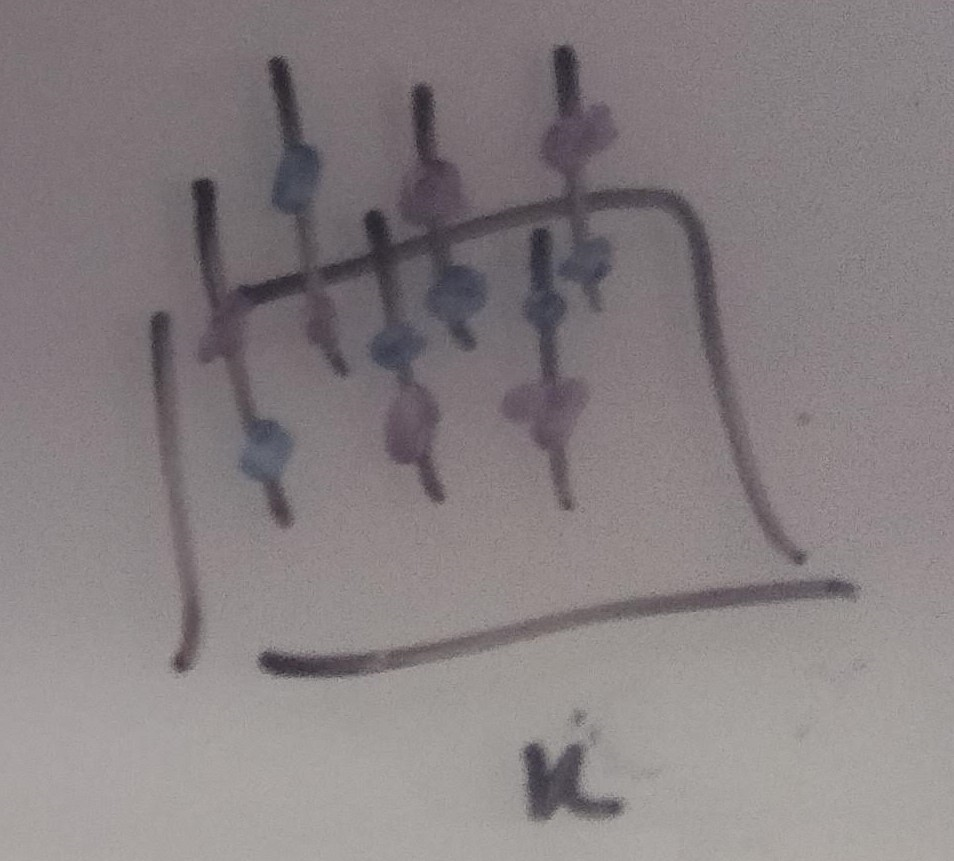
\includegraphics{figures/sections/math/temp_2k.png}
\end{figure}
%% general statement about topology, examples of 0, 1, ....Ks [none triangular things, square/torus, ....], condition on K is that it can be represent as a triangulation of K (can be realized as triangle on K - extra structure that may be arbitrary
%% k is a topological space ....equation soup 




\subsubsection{Fiber Space $F$}
\begin{figure}
    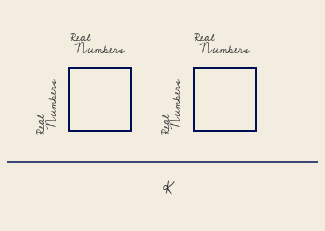
\includegraphics{figures/sections/math/temp_2f.png}
    \label{fig:}
\end{figure}
\begin{figure}
    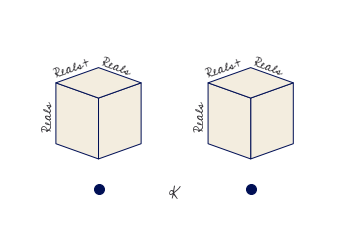
\includegraphics{figures/sections/math/temp_3f.png}
\end{figures}
%%% might 
The fibers $F$ are a topological space embedded in $E$ on which lie the set of all possible values. For example, if $F$ is the interval $[0, 1]$, then $g(k)$ from equation~\ref{eq:sigma} returns a single measurement $x$ in the interval $F$:
\begin{equation}
    \label{eg:goff}
    g(k) = x, \text(where} 0\leq x \leq 1
\end{equation}

The fiber in figure~\ref{fig:temp} is the space of possible temperature values in $\circ$ celsius, ranging from [start, end], similar to the interval $F$ in equation~\ref{eg:goff}. F can be any number of dimensions, for example in figure~\ref{fig:temp_time} time is encoded as a second dimension. Given:
\begin{enumerate}
\item interval of all possible temperarture values $\[T_{min}, T_{max}\]$ 
\item interval of all possible  time values $\[t_{min}, t_{max}\]$
\end{enumerate}

then $F$ is the cross product $F= \[T_{min}, T_{max}\] \times \[t_{min}, t_{max}\]$, and $g(k)$ listed in equation~\ref{eq:sigma} is:
\begin{equation}
g(k) = (x_0, x_1) \text{where} x_0 \in \[T_{min}, T_{max}\], x_1 \in \[t_{min}, t_{max}\]
\end{equation}

Given $F = X_{0} \times X_{1} \times \ldots \times X_{n}$, where $X_{0}, X_{1}, \ldots X_{n}$ are measurement spaces (e.g. ints, floats, colors).
\begin{equation}
g(k) = (x_0, x_1, \ldots x_n) \text{where} x_0 \in X_0, x_1 \in X_1, \ldots x_n \in X_n
\end{equation}

These measurement spaces $X$ are each variables and have the properties of measurement scales, such as Steven's nominal, ordinal, interval, and ratio \cite{stevensTheoryScalesMeasurement1946}





\cite{spivakSIMPLICIALDATABASES}. 



\subsubsection{Subset}
$\Gamma(E)$ is the space of all points in $F$ returned by $\sigma$; therefore the points being visualized in a streaming or animation example can be considered a subset that lives on base space $U$ embedded in $K$ with the same fiber $\iota^*E$ and $\iota^*\sigma$.   

\begin{tikzcd}
    \iota^\ast E \arrow[r, hook] \arrow[d]                                                                       & E \arrow[d, bend right]                       \\
    U \arrow[r, "\iota" description, hook] \arrow[u, "\iota^\ast \sigma" description, bend right, shift right=2] & K \arrow[u, "\sigma" description, bend right]
\end{tikzcd}

\subsection{Prerender Space}
\label{sec:display}

% preamble type intro to displays, examples - displays can include screen, 3D printer, sphereical display, H is the total space of the screen. 11
\begin{figure}[h]
    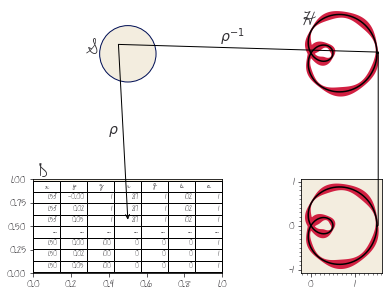
\includegraphics[width=.4\linewidth]{figures/sections/math/render.png}
    \caption{}
    \label{fig:render}
\end{figure}

A physical display space can be thought of sets of $\mathbb{R}^{7}$ tuples, where 
\begin{equation}
    \mathbb{R}^{7} = \{X, Y, Z, R, G, B, A\}
\end{equation}

and the sets correspond to the sections on $\S$, which is the topology of the output of the artist $A$. The space $H$ is a total space representing the predisplay space, with a fiber of $\mathbb{R}^7$ and a base space of $\S$:

\begin{tikzcd}
    \mathbb{R}^{7} \arrow[r, hook] & H \arrow[d, "\pi" description, bend right] \\
                                   & S \arrow[u, "\rho" description, bend right] 
\end{tikzcd}


In the case of 2D screens, the predisplay space is a trivial fiber bundle $H=\mathbb{R}^{7}\times S$. As illustrated in figure~\ref{fig:render}, a region on the screen defined by the corners $(x_1, y_1)$ and $(x_2, y_2)$ maps into a region on a 2-simplex in $S$ defined by $(\alpha_1, \beta_1)$ and $(\alpha_2, \beta_2)$. The function on the simplex $f$ returns the (R, G, B, A) value for that $(\alpha, \beta)$ pair. For a region, 

\begin{equation*}
\rho(S) = \int_{\alpha_1}^{\alpha_2}\int_{\beta_1}^{\beta_2}\int_{z_1}^{z_2}{R, G, B, A}  
\end{equation*}

where the R,G,B,A values are derived from the how the data values are mapped to visual characteristics. The z component of the mapping to $\mathbb{R}^7$ is moved to the integration because this is a trivial space representing a 2D screen; $\rho$ varies depending on $H$. 

%%%pho is paramterized over alpha, beta, which is obtained via pullback lookup from (Hx,Hy)-?(alpha, beta)

\subsection{Artist}
%% include some words about motivation 
\begin{equation}
    A: \Gamma(E) \rightarrow \Gamma(H)
\end{equation}

\subsubsection{Screen to Data}
%%diagram: [data] -Tau->[RGVXYZ]
%%%            \ /\ / 
\begin{tikzcd}
    E \arrow[d, "\pi" description] & H \arrow[d, "\pi" description]                                                 \\
    K \arrow[u, "\sigma" description, bend right] & S \arrow[l, "\xi" description] \arrow[u, "\rho" description, bend right]
\end{tikzcd}

The pullback $\xi$ on $S \rightarrow K$ means that the values in $E$ can be directly mapped to a simplex in $S$, which means there's a mapping from screen space back to the values. 

\begin{tikzcd}
    \xi E \arrow[rr, "\tau" description] \arrow[rd, "\xi \sigma" description, bend right] &     & H \arrow[ld] \\
    & S \arrow[lu, bend right] &             
\end{tikzcd}


\subsubsection{Marks}
%% diagram of connected components/line thing 11-19-20 notes
Bertin describes a location on the plane as the signifying characteristic of a point, measurable length as the signifying characteristic of a line, and measurable size as the signifying characteristic of an area and that in display (pixel) space these are marks \cite{bertinIIPropertiesGraphic2011,carpendaleVisualRepresentationSemiology}. 
\begin{equation}
\begin{tikzcd}
    H \arrow[r, shift left] & S \arrow[l, "\rho(\xi^{-1}(J))", shift left] \arrow[rr, "\xi(s)", shift left] &  & J_{k} =  \{j \in K| \exists \Gamma \text{ s.t. } \Gamma(0)=k \text{ and }\Gamma(1)=j\} \arrow[ll, "\xi^{-1}(J)", shift left]
\end{tikzcd}
\label{eq:mark}
\end{equation}

Each point $s$ in the display space $H$, the mark it belongs to can be found by mapping $s$ back to $K$ via the lookup on S described in section~\ref{sec:display} then taking $\xi(s)$ back to a point on $k \in K$ which lies on the connected component $J \subset K$. To got back to the display space $H$  from the simplacial complex $J$ of the signifier implanted in the mark, the inverse image of $J \in S, \xi^{-1}(J)$ is pushed back to $S$, and then  $\rho(\xi^{-1}(J))$ maps it into $R^{7}$. 



\subsubsection{Visual Characteristics}
Tau can preserves the measurement type properties (group scales)


Tau is fully flexible and can do whatever; knows about fiber & neighborhood of fiber. Can in theory approximate hatching/dashing/etc can be approximated w/ functions and neighborhood of k. 
\subsubsection{Visual Idioms: Equivalance class of artists}
Two artists are equivalent when given data containers $\Gamma(E)$ of the same type, they output the same type of prerender $\Gamma(S)$:
\begin{equation}
    \begin{tikzcd}
        A_{\tau_2}: \arrow[d, shift right=2] & \Gamma(E) \arrow[r] & \Gamma(H) &                                                \\
        A_{\tau_1}: \arrow[u, shift right]   & \Gamma(E) \arrow[r] & \Gamma(H) 
    \end{tikzcd}
\end{equation}

\end{document}